\chapter{Introduction and Motivation}

In times of climate change, the need to reduce greenhouse gas emissions is prevalent. 
One area of interest is carbon dioxide produced via electricity used in data centers. 
For Europe, total usage of electricity for datacenter is placed at 2.7\% in 2020~\webcite{web_bundestag_rechenzentrum}.  
This is projected to increase to 3.4\% in 2030.
However, not all energy is produced equally: while a data center may source its power from the public grid, it itself is sourced from different producers. 
These include high-carbon intensive technologies such as coal and gas but also include low-carbon sources such as wind and solar. 
The latter, follows a diurnal rhythm over the day as shown in Figure \ref{fig:energy_mix}.

As the sun shines more during the day, a bigger part of the total power production comes from solar, reducing the overall \emph{carbon intensity} of the grid.
This can be used for \emph{carbon-aware scheduling}. 
By planning work in data centers to be executed during such low-intensity times, the emissions for a given workload can be reduced.
 
\begin{figure}[H] % holy moly, did he just H this?
    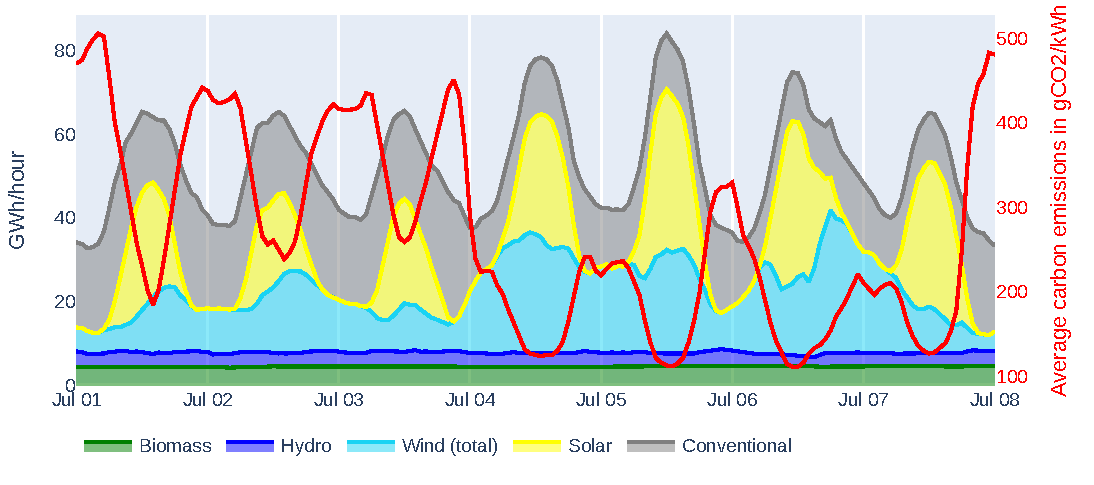
\includegraphics[width=\linewidth]{agorameter/energy_production_week.pdf}
    \caption[short]{Mix of energy production in Germany for the first week of July 2024 with the resulting hourly average carbon emissions per kWh \webcite{web_agora}. Solar production peaks at noon, reducing carbon intensity, creating times, where jobs may be scheduled more carbon efficiently.}
    \label{fig:energy_mix}
\end{figure}

Current work on carbon-aware scheduling focuses on three approaches:
Shifting workloads \emph{temporally}, deferring them until carbon-intensity is lower.
Moving workloads \emph{spatially} by executing them in lower carbon regions.
\emph{Scaling} resources vertically to carbon-intensity~\cite{thiede_carbon_2023,jacob_does_2023}.
Another strategy for executing jobs during low-carbon timeframes is to \emph{suspend \& resume}: a job may be, for example, stopped as carbon intensity is increasing and resumed when a certain threshold is reached. 

One common theme in related work, however, is that the workload models do not include program heterogeneity: while real-world programs may include high-powered times for computation and low-powered times e.g. I/O, this is not reflected in literature. 
Suspending and resuming a workload also carries no overhead in prior work. 

A prominent example of suspendible workloads is machine learning. Currently, there are major pushes to make AI more environmentally friendly \cite{schwartz_green_2019}. 

\paragraph{Structure of this Thesis}

In this work, we will first conduct a structured literature review to outline the state of the art of carbon-aware scheduling. 
We then conduct power measurements on a select machine learning workload.
These will be used to define a new workload model, \modelname{}, that includes startup costs and has phases of different power levels. 
We then modify an existing testbed, GAIA, for our implementation of \programname{}, a carbon scheduling testbed under the changed assumptions.
In the end, we will evaluate how the carbon-emissions of our new heterogeneous jobs with startup costs compare against the workload model used in literature.

\begin{enumerate}
    \item Are there carbon savings under a workload model including resume-overhead and power-heterogeneity?
    \item How does this compare to previous work in the field using the homogeneous model?
    \item Which jobs are better suited for carbon-aware scheduling?
\end{enumerate}
